\section{Problem description}\label{sec:model}

Given a description of the current state of the network, the goal of our algorithm is to produce a new timetable for the trains, keeping in mind what was the original, nominal timetable published to the users. There are, therefore, three main objects that we need to model to provide input data to the algorithm: the first is a description of the \emph{physical network}; the second is the \emph{nominal timetable}, the third is the current status of the trains in the network (called the \emph{forecast timetable}).

\subsection{Network and timetables}\label{ssec:network}

The main tool we use to represent the train network is the \emph{network (di)graph} $\NetGraph = (\Nodes, \Arcs)$. Nodes in $\Nodes$ represent resources. What a resource is can vary greatly and depends mostly on the level of detail we want to achieve when modelling the train network. At a microscopic level, a resource could be a single section of track between two signals, a platform at a station, a junction between tracks, etc. On a macroscopic level, it could be a whole station, or a set of parallel tracks between two stations, etc.

There are, of course, trade-offs between macroscopic and microscopic representations. While the latter will produce a larger graph, using the former will lead us to lose some information. For example, when we represent a set of parallel tracks as a single resource, we can't guarantee that a feasible assignment of trains to the tracks always exists.

Talking about resources rather than more specific railway elements, however, allows us to generalise many aspects of railway networks and even to mix micro- and macroscopic representations in the same graph. This is useful, for example, when the central part of the network is particularly congested and needs a higher level of detail, while peripheral parts are less loaded and can be modelled at a lower resolution.

For example, \Cref{fig:example_macro} shows a macroscopic modelling of a station $S$ and two set of tracks $L$ and $R$. \Cref{fig:example_micro} shows the same station and tracks at a microscopic level: the station has been substituted by three platforms and the generic set of tracks have been replaced by a node for each physical track. Furthermore, connecting tracks have been introduced, to model the connections between the platforms and the tracks. Notice that a solution that was feasible in \Cref{fig:example_macro} might not be feasible in \Cref{fig:example_micro}. For example, a train leaving $P_1$ to reach $R_2$ and a train leaving $P_2$ to reach $R_1$ can't depart at the same time, as they would violate the capacity of $S_{R2}$ (which is $1$), but we wouldn't have been able to rule out this solution just by looking at \Cref{fig:example_macro} and the capacities of the aggregate nodes.

\begin{figure}
	\begin{subfigure}[ht]{\textwidth}
		\begin{center}
			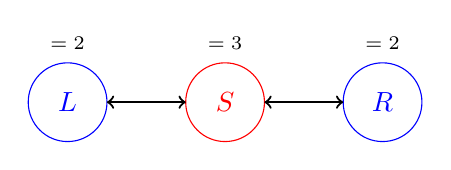
\begin{tikzpicture}
	\draw[blue] (-2,0) circle[radius=0.5] node {$L$};
	\draw[red] (0,0) circle[radius=0.5] node {$S$};
	\draw[blue] (2,0) circle[radius=0.5] node {$R$};
	
	\draw[<->,thick] (-1.5,0) -- (-0.5,0);
	\draw[<->,thick] (0.5,0) -- (1.5,0);
	
	\node at (-2,.75) {\scriptsize$\hardcapacity=2$};
	\node at (0,.75) {\scriptsize$\hardcapacity=3$};
	\node at (2,.75) {\scriptsize$\hardcapacity=2$};
\end{tikzpicture}
		\end{center}
		\caption{Macroscopic representation of station $S$ with tracks $L$ on its left and $R$ on its right.}\label{fig:example_macro}
	\end{subfigure}\vspace{2em}
	\begin{subfigure}[ht]{\textwidth}
		\begin{center}
			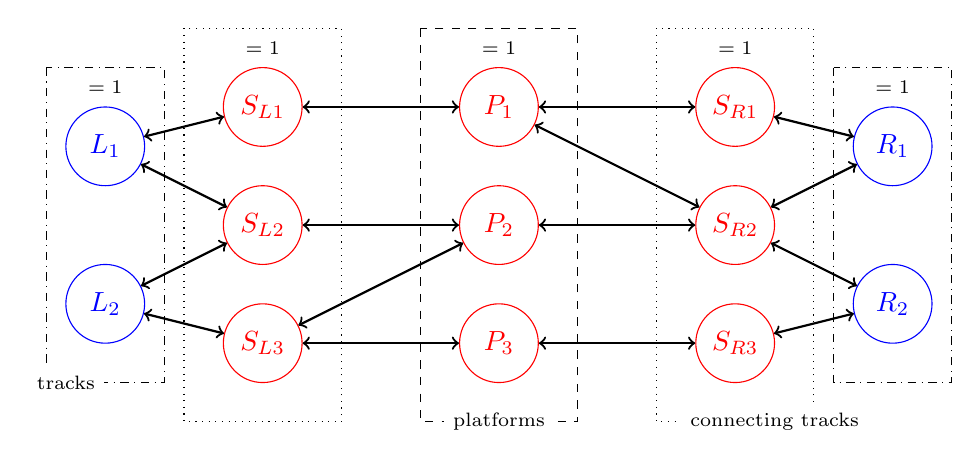
\begin{tikzpicture}
	\tikzstyle{vertex}=[circle,draw,inner sep=0pt, minimum size=1cm]
	
	\node[vertex,blue] at (-5,1) (l1) {$L_1$};
	\node[vertex,blue] at (-5,-1) (l2) {$L_2$};
	
	\node[vertex,red] at (-3,1.5) (sl1) {$S_{L1}$};
	\node[vertex,red] at (-3,0) (sl2) {$S_{L2}$};
	\node[vertex,red] at (-3,-1.5) (sl3) {$S_{L3}$};
	
	\node[vertex,red] at (0,1.5) (p1) {$P_1$};
	\node[vertex,red] at (0,0) (p2) {$P_2$};
	\node[vertex,red] at (0,-1.5) (p3) {$P_3$};
	
	\node[vertex,red] at (3,1.5) (sr1) {$S_{R1}$};
	\node[vertex,red] at (3,0) (sr2) {$S_{R2}$};
	\node[vertex,red] at (3,-1.5) (sr3) {$S_{R3}$};
	
	\node[vertex,blue] at (5,1) (r1) {$R_1$};
	\node[vertex,blue] at (5,-1) (r2) {$R_2$};
	
	\draw[<->,thick] (l1) -- (sl1);
	\draw[<->,thick] (l1) -- (sl2);
	\draw[<->,thick] (l2) -- (sl2);
	\draw[<->,thick] (l2) -- (sl3);
	
	\draw[<->,thick] (sl1) -- (p1);
	\draw[<->,thick] (sl2) -- (p2);
	\draw[<->,thick] (sl3) -- (p2);
	\draw[<->,thick] (sl3) -- (p3);
	
	\draw[<->,thick] (p1) -- (sr1);
	\draw[<->,thick] (p1) -- (sr2);
	\draw[<->,thick] (p2) -- (sr2);
	\draw[<->,thick] (p3) -- (sr3);
	
	\draw[<->,thick] (sr1) -- (r1);
	\draw[<->,thick] (sr2) -- (r1);
	\draw[<->,thick] (sr2) -- (r2);
	\draw[<->,thick] (sr3) -- (r2);
	
	\draw[dashed] (-1,2.5) rectangle (1,-2.5);
	\node[fill=white] at (0,-2.5) {\scriptsize platforms};
	
	\draw[dotted] (-4,2.5) rectangle (-2,-2.5);
	\draw[dotted] (2,2.5) rectangle (4,-2.5);
	\node[fill=white] at (3.5,-2.5) {\scriptsize connecting tracks};
	
	\draw[dashdotted] (-5.75,2) rectangle (-4.25,-2);
	\draw[dashdotted] (4.25,2) rectangle (5.75,-2);
	\node[fill=white] at (-5.5,-2) {\scriptsize tracks};
	
	\node at (-5,1.75) {\scriptsize$\hardcapacity=1$};
	\node at (-3,2.25) {\scriptsize$\hardcapacity=1$};
	\node at (0,2.25) {\scriptsize$\hardcapacity=1$};
	\node at (3,2.25) {\scriptsize$\hardcapacity=1$};
	\node at (5,1.75) {\scriptsize$\hardcapacity=1$};
\end{tikzpicture}
		\end{center}
		\caption{Microscopic representation of the same station as in \Cref{fig:example_macro}, with all platforms and physical tracks modelled explicitly.}\label{fig:example_micro}
	\end{subfigure}
	\vspace{1em}
	\caption{Differences between the micro- and macroscopic representations of a station. $\hardcapacity$ represents the capacity of a resource.}
\end{figure}

We identified certain properties that apply to all resources, no matter what parts of the physical network they represent:
\begin{itemize}
  \item Every node $\node \in \Nodes$ has an ideal (or \emph{soft}) capacity $\softcapacity_\node \in \Nat$ and a \emph{hard} capacity $\hardcapacity_\node \in \Nat$. The capacity of a resource indicates the number of trains that can occupy it at the same time. While the soft capacity can be violated (by possibly paying a certain penalty) the hard capacity cannot be violated under any circumstances. The relation $\softcapacity_\node \leq \hardcapacity_\node$ holds.
  \item Every node $\node \in \Nodes$ also has an associated boolean parameter, $\canovertake_\node \in \{0,1\}$, that indicates whether overtaking and crossing between trains can happen at the node.
\end{itemize}

The arcs in set $\Arcs$ represent the possibility for trains to move from one node to another. Arcs also have capacities, indicating the number of trains that can simultaneously transit from the source to the destination node of the arc: we indicate the capacity of $\arc \in \Arcs$ with $\hardcapacity_\arc \in \Nat$. This quantity is considered as a hard capacity.

The other main actors of a train network are, naturally, trains. Let $\Trains$ be the set of trains and consider the following properties that link together resources and trains:
\begin{itemize}
  \item Given a train $\train \in \Trains$ and a resource $\node \in \Nodes$, we give the minimum and maximum \emph{travel times}, i.e., the minimum and maximum times that $\train$ is allowed to occupy $\node$. We denote these values with $\mintraveltime_{\train,\node}$ and $\maxtraveltime_{\train,\node}$ respectively. The physical meaning of these quantities can vary depending on what the resource models. In case of a section of track, $\mintraveltime_{\train,\node}$ is given by the length of the track and the maximum speed that the train can achieve on that track. On the other hand, in case of a platform, $\mintraveltime_{\train,\node}$ is the dwelling time.
  \item Given a resource $\node \in \Nodes$, we denote with $\headway_\node$ the minimum \emph{headway} at $v$, i.e., the time that must elapse between two trains occupying the resource.
\end{itemize}

The nominal timetable describes the ideal operational status of the network. Each train $\train \in \Trains$ has a predefined path in the network,  denoted as $\trainpath_\train = (\node_1, \node_2, \ldots, \node_{k_\train})$, which is simply a sequence of resources to be visited: $\node_1, \ldots, \node_{k_\train} \in \Nodes$.

For each node in the path of train $\train$, the nominal timetable also provides the times at which the train is supposed to enter and leave the node. These times are denoted as $\intime_{\train,\node_j}$ and $\outtime_{\train,\node_j}$ respectively.

The current train plan describes the network as it is at the present moment --- and as it is forecast to be in the future, given the information available. For this reason, such a plan is also called the \emph{forecast timetable}. In an ideal scenario, the forecast timetable is always equal to the nominal one. In practice, when a disturbance or a disruption occurs, the forecast diverges from the nominal timetable.

The forecast timetable has a formal structure which is similar to that of the nominal timetable: it gives a sequence of nodes that each train must visit, together with the expected in- and out-times. Since both timetables describe the (ideal and real, respectively) situation of the network before the dispatcher takes any decision regarding rerouting, the train paths must be the same in both.

The only new parameters associated with the forecast are, therefore, the in- and out-times. To account for the uncertainty that comes with the real-time situation of the network, we actually give pairs of minimum and maximum possible in- and out-times. These values should be considered as hard values, i.e., the train cannot possibly enter a node before the minimum in-time or after the maximum in-time.

The minimum in- and out-times are denoted, respectively, as $\minintime_{\train,\node_j}$ and $\minouttime_{\train,\node_j}$, for $j = 1, \ldots, k$. The maximum in- and out-times are $\maxintime_{\train,\node_j}$ and $\maxouttime_{\train,\node_j}$.

As we mentioned in \Cref{sec:timetables}, rescheduling a train can involve rerouting it. This means that the dispatcher is allowed to change the path of the train in the network. In our model, we assume that it is only possible to choose detours from a predefined set available for each train. The set of detours associated with train $\train$ is $\Detours_\train$.

A detour is nothing more than a path in the network, so an element $\detour \in \Detours_\train$ contains a sequence of nodes: $\detour = (\node_1, \node_2, \ldots, \node_k)$. We only require that both the first and the last node of the detour are also part of the original train path $\trainpath_\train$. Furthermore, similarly to what we have seen for the current train plan, maximum and minimum in- and out-times are given for each node $\node_j$ of the detour. These are denoted as $\minintime_{\train,\detour,\node_j}$ (minimum in-time), $\maxintime_{\train,\detour,\node_j}$ (maximum in-time), $\minouttime_{\train,\detour,\node_j}$ (minimum out-time), and $\maxouttime_{\train,\detour,\node_j}$ (maximum out-time).

\subsection{Time-space graph}\label{ssec:timespace}

\begin{figure}
	\begin{center}
		\begin{tikzpicture}
	\usetikzlibrary{decorations.pathreplacing}
	
	\node[red] at (-1,5) {$\node_1$};
	\node[red] at (-1,1) {$\node_2$};
	
	\draw[blue,decorate,decoration={brace,mirror,amplitude=10pt}] (-0.25,6.5) -- (-0.25,3.5);
	\draw[blue,decorate,decoration={brace,mirror,amplitude=10pt}] (-0.25,2.5) -- (-0.25,-0.5);
	
	\node[blue] at (0,6) {$\stnode^\textup{L}_1$};
	\node[blue] at (0,4) {$\stnode^\textup{R}_1$};
	\node[blue] at (0,2) {$\stnode^\textup{L}_2$};
	\node[blue] at (0,0) {$\stnode^\textup{R}_2$};
	
	\draw[->,blue] (1.5,7) -- (12,7) node[midway,fill=white] {time};
	
	\foreach \x in {1,...,8}
		\foreach \y in {0,...,3}
			\node at (1.5*\x,2*\y) (n\x\y) {\textopenbullet};
			
	\foreach \x in {1,...,6}
	{
		\pgfmathtruncatemacro{\r}{\x+1};
		\pgfmathtruncatemacro{\s}{\x+2};
		\draw[black!50,->] (n\x3) -- (n\r2);
		\draw[black!50,->] (n\x3) -- (n\s2);
	}
	\draw[black!50,->] (n73) -- (n82);
	
	\foreach \x in {1,...,8}
	{
		\draw[black!50,->] (n\x2) -- (n\x1);
	}
	
	\foreach \x in {1,...,5}
	{
		\pgfmathtruncatemacro{\r}{\x+1};
		\pgfmathtruncatemacro{\s}{\x+3};
		\draw[black!50,->] (n\x1) -- (n\r0);
		\draw[black!50,->] (n\x1) -- (n\s0);
	}
	\draw[black!50,->] (n61) -- (n70);
	\draw[black!50,->] (n71) -- (n80);
\end{tikzpicture}
	\end{center}
	\caption{Example of a portion of time expanded graph.}\label{fig:time_exp}
\end{figure}

The network graph $\NetGraph = (\Nodes, \Arcs)$ introduced in \Cref{ssec:network} does not explicitly model the time component. In this subsection, we present a time-space graph and we construct it starting from $\NetGraph$ and augmenting the number of nodes to take into account time and entry/exit points of nodes of $\Nodes$. Time-expanded graphs have already been used to model railway networks, e.g., in \citet{Caprara2002} and \citet{Cacchiani2010}. The \emph{time-space (di)graph} of a train $\train \in \Trains$ is denoted as $\STGraph^\train = (\STNodes^\train, \STArcs^\train)$ and is obtained in the following way.

For every entry and exit point of every node $\node \in \Nodes$, a node is added to $\STNodes^\train$. The definition of entry and exit point is strongly dependent on the physical resource modelled by $\node$. For example, if $\node$ represents a set of parallel tracks, there will be one entry and one exit point for each track; if $\node$ models a station, there would be an entry and one exit point for every track running through the station. In general, the number of entry and exit point does not need to match (e.g., a station could have more tracks one side than the other). The names \emph{entry} and \emph{exit} are only used to distinguish two physical locations on the resource, but since trains can generally run on a resource in both directions, a specific train could actually enter the resource from one of its exit points and leave it from one of the entry points.

We then need to model time into the graph. In order to do this, we first have to decide a reasonable time horizon and a time discretisation. In practical applications, these values could be provided to the model by the upstream conflict detection system. Notice, though, that the flexibility bundled with our model allows us to use different time discretisations in different parts of the time-space graph: some resources or some time intervals can be modelled with a more precise time discretisation than others. For example, it is possible to have a denser time discretisation for peak times and a sparser one for low-congestion times (e.g., at night). A denser discretisation might also be necessary for short tracks, where the travelling time could be shorter than the standard time interval. Once the time discretisation and the time horizon have been fixed, each node gets one further copy per time instant.

Finally, two dummy nodes $\source^\train$ and $\sink^\train$ are added to each graph $\STGraph^\train$. They represent, respectively, a source and sink node used as the start and end point of the train's path in the graph.

Arcs are created between pairs of nodes $(\stnode_1, \stnode_2) \in \STNodes^\train$ and they are divided in three types. The first type links nodes which represent entry and exit point relative to the same resource $\node \in \Nodes$. Such an arc would model the travelling of a train along the resource modelled by $\node$, when the difference in time instants represents a feasible travelling time for train $\train$.

The second type links nodes which represent entry and exit points of adjacent resources, that is of nodes $\node_1,\node_2 \in \Nodes$ such that $(\node_1,\node_2) \in \Arcs$. Such an arc would model a train that leaves a resource and (instantaneously) reaches a new one.

Finally, the third type links the source and the sink to the other nodes. Let $\sstnode^\train$ and $\estnode^\train$ be the entry points that train $\train$ has to use to access and leave, respectively, its start and end resources. We then add to the arc set $\STArcs^\train$ a:
 \begin{inparaenum}[(a)]
	 \item arcs from $\source^\train$ to nodes of the form $(\sstnode^\train, \timeinstant)$, where $\timeinstant$ is a time instant;
	 \item arcs from nodes of the form $(\estnode^\train, \timeinstant)$ to $\sink^\train$, where $\timeinstant$ is a time instant;
	 \item arcs from nodes of the form $(\stnode, T)$ to $\sink^\train$, where $\stnode$ is any entry or exit point, and $T$ is the last time instant of the time horizon, used to represent a train that could not reach its destination within the time horizon considered.
 \end{inparaenum}

We list the three type of arcs separately and let $\STArcs^\train = \STArcs^{\train,1} \cup \STArcs^{\train,2} \cup \STArcs^{\train,3}$, where the three sets contain, respectively, arcs of the three types listed above.

\Cref{fig:time_exp} shows a portion of a time-expanded graph. Nodes $\stnode^\textup{L}_1$ and $\stnode^\textup{R}_1$ are the left and right extreme points of $\node_1 \in \Nodes$, while nodes $\stnode^\textup{L}_2$ and $\stnode^\textup{R}_2$ are the left and right extreme points of $\node_2 \in \Nodes$. The arcs between $\stnode^\textup{L}_1$ and $\stnode^\textup{R}_1$ represent the traversal of resource $\node_1$ and, analogously, the arcs between $\stnode^\textup{L}_2$ and $\stnode^\textup{R}_2$ represent the traversal of resource $\node_2$. Different arcs having the same source node model the different travelling times associated to different speeds. The vertical arcs between $\stnode^\textup{R}_1$ and $\stnode^\textup{L}_2$ represent the possibility of moving from $\node_1$ to $\node_2$.

The arcs in $\STArcs^{\train,1}$ can be mapped back to the resources and the time intervals they represent in the following way. For each arc $\arc \in \STArcs^{\train,1}$, let $\uresource(\arc) \in \Nodes$ be the underlying resource modelled by the arc; analogously, let $\duresource(\arc) \in \Nodes \times \{ -1, +1 \}$ be the directed underlying resource, used to distinguish the direction in which the resource is being traversed; let $\reslength(\arc)$ be the length of the associated resource $\uresource(\arc)$. Let also $\stime(\arc)$ and $\etime(\arc)$ be the start and end time of arc $\arc$, i.e. the times when the train (respectively) occupies and frees the resource.

\subsection{Constraints}\label{ssec:conflicts}

As defined in \Cref{sec:introduction}, conflicts are those situations that either can't physically happen or that would compromise the safety of operations, and their resolution plays the same role as satisfying a constraint in a Mixed Integer Programme (MIP). In order to give a more precise description of the contraints presented in the rest of this section, we give some mathematical formulation in which we use the notation $x^\train_\arc \in \{0,1\}$ as a variable in a Mixed Integer Programme, having value 1 iff the arc $\arc \in \STArcs^\train$ is part of the path of train $\train$.

Preliminary experiments with solving a compact MIP formulation of real-life instances with a commercial solver have shown that model generation alone can take several minutes, and solving the root node requires more than a day. For this reason, we do not include a complete MIP model for the problem we are presenting. Rather, the notation $x^\train_\arc$ should be seen as a way to describe precisely the constraints taken into account by our algorithm, and how they are reflected on the time-space graph.

Notice, first of all, that a train schedule can be modelled as a path in $\STGraph^\train$, starting in $\source^\train$ and ending in $\sink^\train$ and abiding to the usual flow conservation constraint. Formally, this means that:
\begin{align}
  \sum_{\arc \in \STArcs^{\train,+}(\source^\train)} x_\arc^\train = 1 \\
  \sum_{\arc \in \STArcs^{\train,-}(\sink^\train)} x_\arc^\train = 1 \\
	\sum_{\arc \in \STArcs^{\train,-}(\stnode)} x_\arc^\train =%
  \sum_{\arc \in \STArcs^{\train,+}(\stnode)} x_\arc^\train & \quad &%
	\forall \stnode \in \STNodes^\train \setminus \{ \source^\train, \sink^\train \}
\end{align}
where $\STArcs^{\train,+}(\stnode)$ (resp. $\STArcs^{\train,-}(\stnode)$) is the set of all arcs outgoing from (resp. incoming to) node $\stnode \in \STNodes^\train$.

In this work we deal with the rescheduling of the trains once the conflicts have already been detected and reported, so we will assume that the complete list of conflicts is available together with the current train plan. In other words, the conflict detection system works upstream of our system. This assumption is not restrictive, as a simple linear-time algorithm over the current train plan is able to produce the complete list of conflicts.

The presence of conflicts could be formally detected by checking for violations in (hard) constraints involving the variables $x^\train_\arc$. As we will see in \Cref{ssec:objective_function}, we want to penalise the violation of certain soft constraints. In a MIP model, for example, a hard capacity limit can be enforced via a constraint, whereas the extent of the violation of a soft capacity limit can be penalised, by introducing an auxiliary variable that plays the role of the slack variable relative to the constraint.

\subsubsection{Illegal crossing and overtake}

\begin{figure}
	\begin{center}
		\begin{tikzpicture}
	\usetikzlibrary{decorations.pathreplacing}
	
	\node[red] at (-1,1) {$\node$};
	
	\draw[blue,decorate,decoration={brace,mirror,amplitude=10pt}] (-0.25,2.5) -- (-0.25,-0.5);
	
	\node[blue] at (0,2) {$\stnode_\textup{L}$};
	\node[blue] at (0,0) {$\stnode_\textup{R}$};
	
	\draw[->,blue] (1.5,3) -- (12,3) node[midway,fill=white] {time};
	
	\foreach \x in {1,...,8}
		\foreach \y in {0,...,1}
			\node at (1.5*\x,2*\y) (n\x\y) {\textopenbullet};
			
	\foreach \x in {1,...,5}
	{
		\pgfmathtruncatemacro{\r}{\x+1};
		\pgfmathtruncatemacro{\s}{\x+3};
		\draw[black!50,->] (n\x1) -- (n\r0);
		\draw[black!50,->] (n\x1) -- (n\s0);
	}
	\draw[black!50,->] (n61) -- (n70);
	\draw[black!50,->] (n71) -- (n80);
	
	\draw[red,thick,->] (n41) -- (n50) node[midway,xshift=0.1cm,yshift=0.3cm] {$\train_1$};
	\draw[orange,thick,->] (n31) -- (n60) node[midway,xshift=-0.3cm,yshift=-0.1cm] {$\train_2$};
\end{tikzpicture}
	\end{center}
	\caption{Train $i_1$ overtaking train $i_2$ on resource $v$. Notice how this situation corresponds to crossing arcs in the time-space graph.}\label{fig:overtake}
\end{figure}

An illegal crossing (overtake) describes a situation when a train would cross (overtake) with another one, on a resource $\node$ where this is illegal, i.e. $\canovertake_\node = 0$. An example of overtaking is described in \Cref{fig:overtake}.

An overtake corresponds to the violation of the following constraints: for each train $\train$, each resource $\node$ where overtaking is forbidden, and each arc $\arc \in \STArcs^{\train,1}$ such that $\uresource(\arc) = \node$:
\begin{equation}
  \sum_{\substack{\trainn \in \Trains \\ \trainn \neq \train}}%
  \sum_{\substack{%
    \arc' \in \STArcs^{\trainn,1} \\%
    \duresource(\arc') = \duresource(\arc), \\%
    \stime(\arc') > \stime(\arc), \\%
    \etime(\arc') \leq \etime(\arc)%
  }}%
  x_{\arc'}^\trainn + x_\arc^\train \leq 1 \label{eq:overtake}
\end{equation}
\Cref{eq:overtake} states that train $\trainn$ overtakes train $\train$ on resource $\node$ if $\trainn$ arrives in $\node$ after $\train$, but leaves $\node$ before $\train$, and both trains travel in the same direction.

Analogously, corresponds to the violation of the following contraints: for each train $\train$, each resource $\node$ on which crossing is forbidden, and each arc $\arc \in \STArcs^{\train,1}$ such that $\uresource(\arc) = \node$:
\begin{equation}
  \sum_{\substack{\trainn \in \Trains \\ \trainn \neq \train}}%
  \sum_{\substack{%
    \arc' \in \STArcs^{\trainn,1} \\%
    \uresource(\arc') = \uresource(\arc), \\%
    \duresource(\arc') \neq \duresource(\arc), \\%
    \etime(\arc) \geq \stime(\arc')%
  }}%
  x_{\arc'}^\trainn + x_\arc^\train \leq 1 \label{eq:crossing}
\end{equation}
\Cref{eq:crossing} states that train $\trainn$ crosses train $\train$ on resource $\node$ if $\trainn$ arrives in $\node$ before $\train$ has left, and the two trains travel in opposite directions.

\subsubsection{Capacity violation}

A capacity violation occurs when the number of trains simultaneously occupying a resource is greater of the hard capacity of the resource. Such a conflict corresponds to a violated inequality of the following type:
\begin{equation}
  \sum_{\train \in \Trains}%
  \sum_{\substack{%
    \arc \in \STArcs^\train \\%
    \uresource(\arc) = \node, \\%
    \stime(\arc) \leq \timeinstant, \\%
    \etime(\arc) \geq \timeinstant%
  }}%
  x_\arc^\train \leq \hardcapacity_\node
\end{equation}
for each resource $\node$ and each time instant $\timeinstant$, where we remind that $\hardcapacity_\node$ is the hard capacity of resource $\node$.

\subsubsection{Headway violation}

Such a conflict occurs when a train occupies a resource that has been occupied by another train, and not enough time has elapsed between the first train leaving the resource and the second one entering it. For each train $\train \in \Trains$ and each arc $\arc \in \STArcs^{\train,1}$ corresponding to a resource $\uresource(\arc)$ on which crossing and overtaking is forbidden ($\canovertake_{\uresource(\arc)} = 0$, as otherwise the headway must not be respected), a headway conflict corresponds to a violated constraint:
\begin{equation}
	\sum_{\substack{%
		\trainn \in \Trains \\%
		\trainn \neq \train%
	}}%
	\sum_{\substack{%
		\arc' \in \STArcs^{\trainn,1} \\%
		\uresource(\arc') = \uresource(\arc) \\%
		\etime(\arc') \geq \stime(\arc) - \headway_{\resource(\arc)} \\%
		\stime(\arc') \leq \etime(\arc) + \headway_{\resource(\arc)}%
	}}%
	x_{\arc'}^\trainn + x_\arc^\train \leq 1
\end{equation}

\subsubsection{Time dependencies}\label{ssec:time_dependencies}

Avoiding the conflicts described in the previous subsection is usually enough to come up with a new plan that allows safe operations and limits the deviations from the nominal timetable. Unfortunately, this is not always enough to provide a holistic, good solution.

Consider, for example, a passenger on a delayed train that risks missing his connection. From his point of view, a solution that also delays his next train (to ``wait for him'') is preferable to a solution that does not. But from a train operator's point of view, a solution that does not delay the second train may be considered better, since no delay is better than some delay.

Then, if the train operator's \emph{service intention} is, for example, ``moving passengers from A to B'' (even at the cost of increasing the overall delay, to some extent), this should be taken into account by the rescheduling algorithm.

In order to take into account service intentions, we introduce the concept of \emph{time dependencies} (\citet{Caimi2011}).
A time dependency is a relationship of precedence between two events happening in the network. For example, a time dependency could mandate that the event ``train $\train_1$ leaves node $\node$'' can only happen a certain time after the event ``train $\train_2$ arrives at node $\node$''; intuitively, we would say that train $\train_1$ needs to wait for train $\train_2$ at node $\node$.

\begin{figure}
	\begin{center}
		\begin{tikzpicture}
	\usetikzlibrary{decorations.pathreplacing}
	\usetikzlibrary{positioning}
	
	\node[red] at (-1,3) {$\node$};
	
	\draw[blue,decorate,decoration={brace,mirror,amplitude=10pt}] (-0.25,6.5) -- (-0.25,-0.5);
	
	\node[blue] at (0,6) {$\stnode^\textup{L}_1$};
	\node[blue] at (0,4) {$\stnode^\textup{L}_2$};
	\node[blue] at (0,2) {$\stnode^\textup{R}_1$};
	\node[blue] at (0,0) {$\stnode^\textup{R}_2$};
	
	\draw[->,blue] (1.5,7) -- (12,7) node[midway,fill=white] {time};
	
	\foreach \x in {1,...,8} {
		\foreach \y in {0,...,3} {
			\ifthenelse{6 = \x \AND 2 = \y}{}{\node at (1.5*\x,2*\y) (n\x\y) {\textopenbullet};}
		}
	}
	
	\tikzstyle{relevant}=[circle,fill,minimum size=0.25cm,inner sep=0pt];
	\node[relevant,red] at (1.5,6) (arr1) {};
	\node[relevant,red] at (9,2) (dep1) {};
	\node[relevant,orange] at (4.5,4) (arr2) {};
	\node[relevant,orange] at (10.5,0) (dep2) {};

	\node[red,above=0.025cm of n13] {Arrival of $\train_1$};
	\node[red,above=0.02cm of n61,xshift=1.275cm] {Departure of $\train_1$};
	\node[orange,below=0.025cm of n32,xshift=-0.75cm] {Arrival of $\train_2$};
	\node[orange,above=0.025cm of n70,xshift=1cm] {Departure of $\train_2$};

	\draw[red,thick,->] (n13) -- (n61);
	\draw[orange,thick,->] (n32) -- (n70);
	
	\draw (n32) -- (n33);
	\draw (n61) -- (n63);
	
	\draw[<->] (4.5,5) -- (9,5) node[midway,fill=white] {\scriptsize Resolution time};
\end{tikzpicture}
	\end{center}
	\caption{Resolution time of a time dependency between the arrival of train $\train_2$ and the departure of train $\train_1$ at a station.}\label{fig:dependency}
\end{figure}

A service intention can merely suggest a precedence between events, as in the case of passenger connections: it is preferable that the connection is kept, but this ``promise'' can be broken in order to improve the overall quality of service. On the other hand, the precedence can also be mandatory, as in the case of two trains that share crew or rolling stock.

Let $\Dependencies$ be the set of time dependencies. We associate to each element $\dependency \in \Dependencies$ the following values:
\begin{itemize}
  \item The two trains $\train_{\dependency,1},\train_{\dependency,2}$ involved in the dependency.
  \item The two resources $\node_{\dependency,1},\node_{\dependency,2}$ at which the linked events need to take place, respectively.
  \item Two parameters $\dependencytype_{\dependency,1},\dependencytype_{\dependency,2} \in \{0,1\}$ that take value $0$ if the corresponding event is an arrival or value $1$ if it is a departure.
  \item A parameter $\mandatory_\dependency \in \{0,1\}$ that takes value $1$ iff the dependency is mandatory.
  \item The minimum and maximum resolution time, $\minrestime_\dependency$ and $\maxrestime_\dependency$. The dependency is considered satisfied if the two events take place at least $\minrestime_\dependency$ and at most $\maxrestime_\dependency$ time units apart.
  \item For non-mandatory (also called \emph{logical}) time dependencies, we give a maximum waiting time $\waittime_\dependency$. The dependency must be satisfied if it is possible to do so by introducing at most $\waittime_\dependency$ time units of delay. If this cannot be done, the dependency can either be satisfied or not. For example, in the case of a connection between two trains, we might require that a train waits for the other at most $\waittime_\dependency$ time units. If the required wait is greater, the train can decide to break the connection.
\end{itemize}

\Cref{fig:dependency} shows an example in which train $\train_1$ stays at station $\node$ for three time intervals after the arrival of train $\train_2$, presumably to \emph{wait} for passengers travelling on $\train_2$. The resources $\stnode_k^\textup{L},\stnode_k^\textup{R}$ represent entry and exit points of two platform at the station ($k = 1,2$).

The violation of a mandatory time dependency $\dependency \in \Dependencies$ can be detected as follows. Assume wlog that the event relative to train $\train_{\dependency,1}$ needs to take place before the event relative to train $\train_{\dependency,2}$. For $k = 1,2$ and $\arc \in \STArcs^{\train_{\dependency,k},1}$ such that $\uresource(\arc) = \node_{\dependency,k}$, consider the parameter:
\begin{equation*}
  \deptime_{\dependency,k}(\arc) =  \begin{cases}
                                      \stime(\arc) & \text{ if } \dependencytype_{\dependency,k} = 1 \\
                                      \etime(\arc) & \text{ if } \dependencytype_{\dependency,k} = 0
                                    \end{cases}
\end{equation*}
  We can then formulate the corresponding constraint:
\begin{equation}
  \minrestime_\dependency \leq%
  \sum_{\substack{%
    \arc \in \STArcs^{\train_{\dependency,2},1} \\%
    \uresource(\arc) = \node_{\dependency,2}%
  }}%
  x_\arc^\train \deptime_{\dependency,2}(\arc) -
  \sum_{\substack{%
    \arc \in \STArcs^{\train_{\dependency,1},1} \\%
    \uresource(\arc) = \node_{\dependency,1}%
  }}%
  x_\arc^\train \deptime_{\dependency,1}(\arc)%
  \leq \maxrestime_\dependency
\end{equation}

\subsubsection{Split and merge}

Similar to time dependencies are split and merge operations. These are events in which the trains that enter a node are not the same that leave it. They model real-life operations such as decoupling some cars from a train, so that they can get a new locomotive and proceed to a different destination.

In the most general version, any number of trains can enter a certain node and any number of trains can leave it, so a split/merge is identified by a node $\node \in \Nodes$ and two sets of trains $\Trains_1,\Trains_2 \subset \Trains$ that represent in-trains and out-trains. The out-trains can leave the node only after a certain amount of time has passed since the last in-train reached it. This time accounts, in practice, for the time necessary to perform any physical coupling and decoupling, or to change crew or rolling stock. Special cases of split/merge operations are:
\begin{itemize}
	\item \emph{Split}, when one train enters the node, and two or more exit it.
	\item \emph{Merge}, when more than one train enter the node, and only one exits it.
	\item \emph{Rename}, when one train enters the node and one train exits it.
\end{itemize}
In case of split/merge events, the node's capacity is not considered, as it is assumed that it is always feasible for the event to take place in the node specified. Finally, note that these events are mandatory: for example, it is not possible that a train will be detoured around a node in which it has to undergo a split.

In the following we show how a split or merge operation can be modelled in terms of mandatory time dependencies; in this way, the conflict resulting from a missed split or merge can be detected by checking for the violation of the corresponding time dependency constraint. For example, if train $\train$ needs to be split into trains $\train', \train''$ at resource $\node$, then said resource will be set as the destination of $\train$ and the origin of $\train'$ and $\train''$. Furthermore, two dependencies will be created:
\begin{itemize}
	\item $\dependency' \in \Dependencies$ links trains $\train$ and $\train'$ and has: $\train_{\dependency',1} = \train, \train_{\dependency',2} = \train'$; $\node_{\dependency',1} = \node_{\dependency',2} = \node$; $\dependencytype_{\dependency',1} = 0, \dependencytype_{\dependency',2} = 1$; $\mandatory_{\dependency'} = 1$; $\minrestime_{\dependency'}$ will be the time needed to perform the split operation; $\maxrestime_{\dependency'}$ will be the maximum time allowed for the split to take place, if any.
	\item $\dependency'' \in \Dependencies$, analogously links trains $\train$ and $\train''$.
\end{itemize}

\subsubsection{Maximum and minimum entry, exit, and travel times}

Maximum and minimum entry, exit, and travel times can be enforced by removing from the graphs $\STGraph^\train$ those nodes that would correspond to an infeasible (resource, time) couple. For example, if a train $\train \in \Trains$ cannot enter resource $\node$ before time $\timeinstant$, all nodes of $\STNodes^\train$ corresponding to resource $\node$ at a time $t' < t$ can be removed from the graph. Analogously, if the minimum travel time along a resource $\node$ is $\timeinstant$, all arcs $\arc \in \STArcs^{\train,1}$ such that $\etime(\arc) - \stime(\arc) < \timeinstant$ can be removed.

\subsection{Objective function}\label{ssec:objective_function}

The objective value can be written as a function of the paths in the time-space graphs, and therefore of $\vec{x} = (x_\arc^\train)$, in the following way:
\begin{equation}
  f(\vec{x}) = f_1(\vec{x}) + f_2(\vec{x}) + f_3(\vec{x}) + f_4(\vec{x}) \label{eq:objf}
\end{equation}
The four components correspond to delays, logical dependency breaking, soft capacity violations, and the use of detours. Each of these components represents a sum of penalties that quantify how undesirable it is to incur in the corresponding violations. The penalty, therefore, is not only limited to represent the economical disadvantage of taking a particular decision (e.g., increased energy consumption) but can also represent intangible values, such as customer satisfaction. In the following, we analyse these four components.

\subsubsection{Delays}

In the nominal timetable, we associated to each train $\train$ and each resource $\node_j$ in the train's path, an ideal in-time $\intime_{\train, \node_j}$ and an ideal out-time $\outtime_{\train, \node_j}$. Any deviation from these times can be penalised, by considering two piecewise-linear functions that respectively assign a cost to delays in arriving at and departing from the resource. These penalty functions are denoted as $\indelaypenalty_{\train,\node_j}(\cdot)$ and $\outdelaypenalty_{\train, \node_j}(\cdot)$.

Notice that this general definition allows us to assign different penalty profiles to different resources: for example, if some resource is considered critical for a train, we can assign a higher penalty to delays at that resource. The function can also operate on negative delays, allowing us to penalise trains that arrive at a node with excessive advance. Finally, further flexibility is bundled in the piecewise-linear nature of the function: for example, we might want to have a penalty that grows linearly with the delay up to a certain point, after which a big flat penalty is assigned, as any further delay does not worsen the situation any more. This could be achieved with a penalty profile such as that in \Cref{fig:example_penalty}.

\begin{figure}
  \begin{center}
    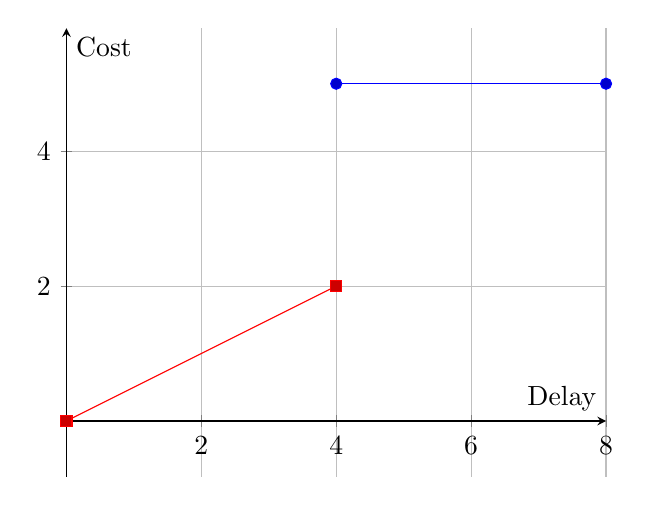
\begin{tikzpicture}
  \begin{axis}[axis lines = middle, axis equal, grid = both, xlabel = {Delay}, ylabel = {Cost}]
    \addplot coordinates{(0,0) (4,2)};
    \pgfplotsset{cycle list shift=-1} % Re-use the same style as the first plot
    \addplot coordinates{(4,5) (8,5)};
  \end{axis}
\end{tikzpicture}
  \end{center}
  \caption{Example of a penalty profile for the arrival of a train at a certain resource, with a ``jump'' in cost if the delay is greater than 4 time units.}
  \label{fig:example_penalty}
\end{figure}

\subsubsection{Dependency breaking}

As we mentioned in \Cref{ssec:time_dependencies}, logical dependencies are not mandatory and therefore we can decide to break them. In our implementation, when such a dependency $\dependency \in \Dependencies$ is broken, we pay a penalty $\dependencypenalty_\dependency$. (Notice that, in principle, a piecewise linear function could be used, as done for delays.)

\subsubsection{Capacity violations}

When we violate the soft capacity $\softcapacity_\node$ of a resource $\node$, we pay a penalty $\capacitypenalty_\node$. In our implementation, this penalty remains the same no matter how big the capacity violation is. (Notice that, in principle, a piecewise linear function could be used in this case too.)

\subsubsection{Detours}

Finally, a fixed penalty $\detourpenalty_{\detour}$ is paid when a train $i$ is re-routed along a detour $\detour \in \Detours_\train$. This penalty takes into account all the costs (economical or otherwise) incurred because of the rerouting. Dependency breaking and capacity violations are calculated separately when a detour is taken. If some node of the detour can be naturally mapped to nodes of the original path, the delay penalty can also be calculated. For example, if the detour consists of a platform change at a station, we can naturally assign to the new platform the in- and out-times at the old platform.

The penalty $\detourpenalty_{\detour}$ should be considered as a fixed cost incurred by the mere fact of having rerouted the train. It can include both \emph{real} and \emph{virtual} costs. For example, if the detour consist of a path longer than the original one, there would be increased energy costs. But if the detour also excludes a station, there would be a much increased passenger dissatisfaction. Therefore, the magnitude of the penalty depends on the type of detour: a platform change will have a small associated penalty, while a major change in the train's path will be associated with a bigger penalty.

\subsubsection{Other terms}\label{sssec:other_terms}

Even though in the present work we only consider the four components discussed above, further terms can be easily introduced in the objective function to take into account other indicators. For example:
\begin{itemize}
	\item Number of modifications with respect to the nominal timetable, eventually weighted differently depending on the nodes or trains involved. This could be done to make sure that the new timetable does not disrupt too much the current operations (i.e., changes too many train paths) just to save a few seconds of overall delay.
	\item Increased travel time on resources, eventually involving a piecewise-linear penalty profile. This term would help avoiding unnecessary stops or excessive brake-accelerate cycles, for increased passenger comfort and reduced energy consumption.
\end{itemize}
